% !TEX encoding = UTF-8 Unicode

\documentclass[a4paper]{article}

\usepackage{color}
\usepackage{url}
\usepackage[utf8]{inputenc}
\usepackage{graphicx}

\usepackage[english]{babel}

\usepackage[unicode]{hyperref}
\usepackage{amsmath}
\usepackage{amsthm}
\usepackage{amssymb}
\hypersetup{colorlinks,citecolor=green,filecolor=green,linkcolor=blue,urlcolor=blue}
\usepackage[title]{appendix}
\usepackage{float}
\usepackage[graphicx]{realboxes}
\usepackage[font=small,labelfont=bf]{caption}
\usepackage{chngcntr}
\counterwithin{figure}{section}
\usepackage{listings}
\usepackage{textcomp}
\usepackage{xcolor}
\lstset {
    language=Java,
    frame=none,
    %xleftmargin=-.25in,
    %xrightmargin=.25in
    framesep=10pt,
    tabsize=4,
    showstringspaces=false,
    upquote=true,
    commentstyle=\color{commentgreen},
    keywordstyle=\color{orange},
    stringstyle=\color{red},
    basicstyle=\small\ttfamily,
    emph={int,char,double,float,unsigned,void,bool},
    emphstyle={\color{blue}},
    escapechar=\&,
    classoffset=1,
    morekeywords={>,<,.,;,,,-,!,=,~},
    keywordstyle=\color{weborange},
    classoffset=0,
    breaklines=true
}

\theoremstyle{plain}
\newtheorem{thm}{Teorema}[section]
\theoremstyle{definition}
\newtheorem{defn}[thm]{Definition}
\newtheorem{exmp}[thm]{Example}
\newtheorem{assn}[thm]{Assumption}
\newtheorem{obsn}[thm]{Observation}

\usepackage[font=scriptsize,labelfont=bf]{caption}


\begin{document}

\title{Bugfixing using valid examples\\ \small{Software Verification course team project\\Faculty of Mathematics, Belgrade}}

\author{\href{mailto:mi14031@matf.bg.ac.rs}{Ivan Ristović}, \href{mailto:mi14042@matf.bg.ac.rs}{Milana Kovačević}, \href{mailto:mi14207@matf.bg.ac.rs}{Strahinja Stanojević}}
\date{September 2018.}

\maketitle

\setcounter{tocdepth}{1}

\abstract{
    We have been tasked with creating a program which will compare two given code snippets - one of which will be used as a specification whereas the other one will semantically differ from the specification - and synthesize a new code snippet which will use the ``invalid'' snippet as the base, but edited to fit the specification. Since it has already been proven that the semantical code comparison problem is indecisive (Halting problem), there is no way to successfully give an answer for all code snippets. However, some subsets of the code snipper space can be tested and even though in some cases we cannot say for certain if what we have found is a bug or not we can provide a false-positive warning. The algorithm we use to compare the two requires mathing and traversing the abstract syntax trees of both codes. For the task of matching code elements we are using GumTree API and as for the traversal we decided to use the JDT Core DOM API which unfortunately limits us to only Java code snippets.
}


\tableofcontents
\newpage

\section{Problem formulation}
\label{sec:Formulation}

Instead of writing a long formulation of the problem at hand we will rather provide a series of examples which will serve as an illustration and hopefully give the reader enough information to grasp the matter without formal definitions \footnote{Some of the definitions would include semantical equivallence of the two code snippets, which would most probably be hard to formulate and even then would probably be ambiguous.}.

\begin{exmp}
\textit{Let's take a look at the following code snippets:}

\begin{tabular}{ p{4.5cm} p{4.5cm} }
\begin{lstlisting}
int foo1()
{
    int x = 1, a = 2;
    return x + a;
}
\end{lstlisting}
&
\begin{lstlisting}
int foo2()
{
    int x = 0, a = 2;
    return x + a;
}
\end{lstlisting}
\end{tabular}

\textit{These two snippets are clearly semantically different, because the \texttt{foo2} function has different value of \texttt{x} variable than function \texttt{foo1}. If we wish to synthesize a fix for the given example pair, we would just replace the initializer for variable \texttt{x} in function \texttt{foo2}  from $0$ to $1$.}
\qed
\end{exmp}

We have seen a very simple example which has a simple solution. The problem, however, gets much more complex as new code structures emerge, such as branching and loops. Also, reader might have noticed that semantical similarity has nothing to do with syntactic similarity.

\begin{exmp}
\textit{Suppose we are given two code snippets, as before:}

\begin{tabular}{ p{4.5cm} p{4.5cm} }
\begin{lstlisting}
int fooEq1()
{
    int x = 1;
    int a = 2;
    return x + a + 1;
}
\end{lstlisting}
&
\begin{lstlisting}
int fooEq2()
{
    return 4;
}
\end{lstlisting}
\end{tabular}

\textit{In this example the syntactic difference is enormous, seeing as the second function has no variables declared and has a single statement, whereas the first one has variables defined and has three statements. Both functions, however, evaluate to the same result: $4$.}
\qed
\label{exmp:DeleteExmp}
\end{exmp}

One might think that in most cases comparing the return values should be sufficient. While that might be true in most cases, the following example proves that, in general, this statement does not hold.

\begin{exmp}
\textit{Side effects like these have an enormous impact on the difficulty of the problem at hand:}

\begin{tabular}{ p{4.5cm} p{4.5cm} }
\begin{lstlisting}
int fooSideEff()
{
    println("Hello!");
    return 1;
}
\end{lstlisting}
&
\begin{lstlisting}
int foo()
{
    return 1;
}
\end{lstlisting}
\end{tabular}

\textit{There is no way to determine for any external function whether it has a side effect or not since we do not have access to it's source code. Therefore, side effects (as well as some other constructs) have been excluded from the analysis - we will specify in the following chapters exactly what code constructs have been excluded or what pre-assumptions were made about the given code snippets.}
\qed
\end{exmp}

\begin{exmp}
\textit{Examples like these though, can be checked and verified to be equivallent even though there are side effects present in the function \texttt{anotherFooEq2}.}

\begin{tabular}{ p{4.5cm} p{4.5cm} }
\begin{lstlisting}
int anotherFooEq1()
{
    int x = 0;
    x += 3;
    return x;
}
\end{lstlisting}
&
\begin{lstlisting}
int anotherFooEq2()
{
    int a = 0;
    a++;
    a++;
    ++a;
    return a;
}
\end{lstlisting}
\label{exmp:PlusPlusExample}
\end{tabular}

\textit{The behavior of \texttt{a++} and \texttt{++a} is exactly the same as long as the value of that expression is not used in that same statement. In this case, it is equivallent to \texttt{a += 1}.}
\qed
\end{exmp}

\begin{exmp}
\textit{We should note that, in general, there is no way of telling whether the execution will reach certain branches of the code due to the lack of determinism if we are to include the user input into the problem:}

\begin{tabular}{ p{4.5cm} p{4.5cm} }
\begin{lstlisting}
int ambFoo1(int x)
{
    return x >= 0
        ? 1
        : 0;
}
\end{lstlisting}
&
\begin{lstlisting}
int ambFoo2(int y)
{
    return y % 2;
}
\end{lstlisting}
\end{tabular}

\textit{These functions are definitely semantically different, but if the caller function always invokes functions with argument $1$, their return values will be the same:}

\begin{tabular}{ p{4.5cm} p{4.5cm} }
\begin{lstlisting}
void wrapper1()
{
    int x;
    x = ambFoo1(1);

    if (x == 1)
        // ...
}
\end{lstlisting}
&
\begin{lstlisting}
void wrapper2()
{
    int x;
    x = ambFoo2(1);

    if (x == 1)
        // ...
}
\end{lstlisting}
\end{tabular}

\qed
\end{exmp}

In the following chapters we will extend the example set with more complicated examples and describe our approach of semantical testing. We will also be using AST representation (see chapter \ref{sec:AST}) instead of plain code analysis.

\section{Assumptions and limitations}
\label{sec:AssumptionsAndLimitations}

In the previous chapter we have shown how certain code structures (loops for example) can be hard to analyze. Therefore we have set a certain number of assumptions on the input code snippets:

\begin{itemize}
    \item All variables have to be initialized before their use
    \item All functions are assumed not to have side effects
    \item Branching condition value needs to be known at compile-time
\end{itemize}

Apart from these assumptions, we have ignored the following in order to make the problem easier:

\begin{itemize}
    \item All data types except int
    \item All code constructs except declarations, assignments, branching statements and arithmetic operators
\end{itemize}


\cite{DBLP:conf/kbse/FalleriMBMM14}

\section{Abstract Syntax Trees}
\label{sec:AST}

Instead of analyzing the code on the higher level or using some internal representation between assembly and high-level code, we have decided to use the \emph{Abstract syntax trees} (\emph{AST} from now on).

\begin{defn}
    An \emph{abstract syntax tree} is a tree representation of the abstract syntactic structure of source code written in a programming language. Each node of the tree denotes a construct occurring in the source code.
\end{defn}

\begin{exmp}
    \textit{Consider the following code snippet:}

    \begin{lstlisting}
    while (x < 20) {
        x = x + y * 2
    }
    \end{lstlisting}

    \textit{The appropriate AST can be seen on figure \ref{fig:WhileAST}.}
\end{exmp}

\begin{figure}
    \centering
    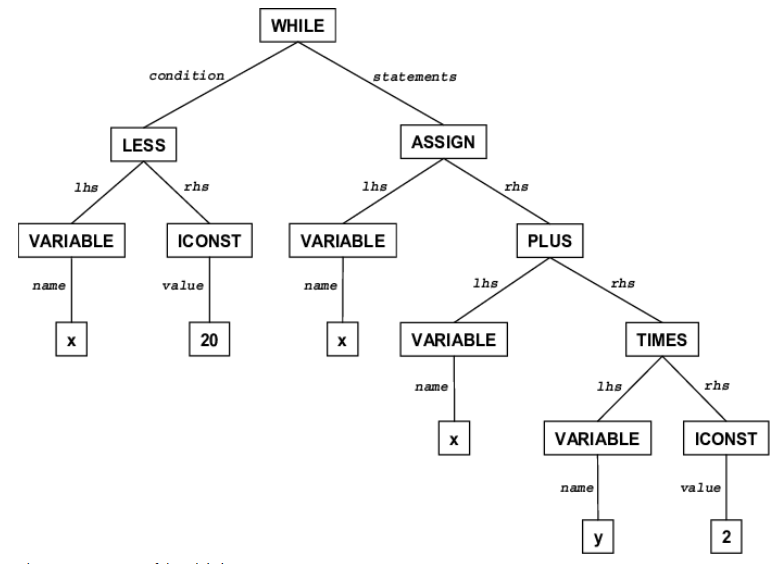
\includegraphics[scale=0.6]{res/WhileAST.PNG}
    \caption{AST for the while loop}
    \label{fig:WhileAST}
\end{figure}

Using the AST instead of the pure code has many advantages. Namely, different code snippets might have the same AST representation which itself does the job of semantical analysis. This is a rare case though, however it is still easier to compare the trees instead of code samples because the tree structure does not contain redundancies like whitespace for example. Also, there exist libraries for AST creation which we use and describe in the following chapter.

\section{Additional tools used}
\label{sec:Tools}

\cite{DBLP:conf/kbse/FalleriMBMM14}

\section{The analysis algorithm}
\label{sec:Algorithm}

We start off by creating two ASTs, one for each code snipet. The first task is to use matchers to find matching tree nodes. Using the GumTree API, we compute the actions required to create the second tree from the first. If those actions contain only variable name updates, then it is safe to say that the trees are equivallent and that the snippets are semantically equivalelnt. If there are insert or delete actions present, one might be tempted to report them as a difference and automatically assume that the actions needed to be done are reverse of those found in order to ``fix'' the second code. As shown in example \ref{exmp:PlusPlusExample}, this is the wrong way of handling the problem at hand.

The second approach is to phrase the semantical equivallence in a different way. This brings us to per-block variable analysis. We assume the following is true for any given code snippet:

\bigskip
\begin{assn}
    Semantically equivallent code snippets have the same variable values at the end of each block.
\end{assn}
\bigskip

To illustrate this, we give an example and explain how we collect and compare variable values for each block.

\begin{exmp}
\bigskip
\textit{Consider the following code snippets:}

\begin{tabular}{ p{4.5cm} p{4.5cm} }
\begin{lstlisting}
int x = 1;
int foo()
{
    int a = 5;

    if (a > 3) {
        x = 2;
    }

    int c = 1;

    if (a > 3) {
        c = 2;
    }
}
\end{lstlisting}
&
\begin{lstlisting}
int y = 1;
int foo2()
{
    int a = 2;

    if (a < 3) {
        y = 2;
    }

    int c = 1;

    if (a < 3) {
        c = 2;
    }
}
\end{lstlisting}
\end{tabular}

\bigskip
\textit{Let's analyze the first snippet ``per-block'':}
\bigskip

\begin{lstlisting}
// Block depth 0, ordinal 1
int x = 1;

int foo()
{
    // Block depth 1, ordinal 1
    // Vars passed: x = 1

    int a = 5;

    if (a > 3) {
        // Block depth 2, ordinal 1
        x = 2;
        // End of block: Update x in parent
    }

    // x = 2 here because of the update

    int c = 1;
    if (a > 3) {
        // Block depth 2, ordinal 2
        c = 2;
        // End of block: Update c in parent
    }

    // Vars: x = 2, a = 5, c = 2
    // End of block: Update x in parent
}

// End of root block: x = 2
\end{lstlisting}

\bigskip
\textit{Using the above information, we create the variable map:}
\bigskip

\begin{table}[H]
\centering
\begin{tabular}{ | c | c | c |}
    \hline
    Block depth & Block ordinal & Variables \\
    \hline
    0 & 1 & x \\
    1 & 1 & x, a, c \\
    2 & 1 & x, a \\
    2 & 2 & x, a, c \\
    \hline
\end{tabular}
\end{table}

\bigskip
\textit{The variable values are stored per each block and each update in the child block will be propagated to the parent block when the end of the child block is reached. Using this variable map as a model, we do the same for the second code snippet. Also, note that renamed variables are not a problem - the matcher will give the update pairs before analysis, in this case (x, y) will be an update pair.}
\bigskip

\begin{lstlisting}
// Block depth 0, ordinal 1
int y = 1;  // Matches to x

int foo()
{
    // Block depth 1, ordinal 1
    // Vars passed: y = 1

    int a = 2;

    if (a < 3) {
        // Block depth 2, ordinal 1
        y = 2;
        // End of block: Update y in parent
    }

    // y = 2 here because of the update

    int c = 1;
    if (a < 3) {
        // Block depth 2, ordinal 2
        c = 2;
        // End of block: Update c in parent
    }

    // Vars: y = 2, a = 2, c = 2
    // Conflict found: a = 5 in source, but found a = 2
    // End of block: Update y in parent
}

// End of root block: y = 2
\end{lstlisting}

\bigskip
\textit{The above algorithm does not take into account what actions are done in a block, as long as the end result of the block is the same - i.e. the variables have the same end-value.}
\qed
\end{exmp}

The pseudo code of the algorithm can be seen in figure \ref{fig:AnalysisAlg}. Returned conflicts can be used to either list or repare the code. For now we are just listing the conflicts.

\begin{figure}[H]
\centering
\begin{lstlisting}
Analyze(tree1: AST, tree2: AST)
begin
    if (CreateMatcher(tree1, tree2).OnlyUpdateActionsFound()):
        /* We have found only rename actions */
        print("Given snippets are equivallent")
        return

    /* In general case, traverse the first tree */
    vmap = tree1.TraverseAndRecordVars()

    /* Traverse the second tree and compare vars per block */
    conflicts = tree2.TraverseAndCompareVars(vmap)

    foreach (conflict in conflicts):
        print(conflict.Details)
end
\end{lstlisting}
\caption{Our analysis algorithm in pseudocode}
\label{fig:AnalysisAlg}
\end{figure}


\addcontentsline{toc}{section}{References}
\bibliography{references}
\bibliographystyle{plain}

%\begin{appendices}
%\input{parts/???}
%\end{appendices}

\end{document}
